\subsection{SRCNN}
Partimo del método descrito en \cite{SRCNN}, en el cual se menciona una red que cuente con al menos 3 capas convolucionales, de
manera que la primer capa se encargue de extraer los parches de baja resolución, la(s) capa(s) intermedias realizan el mapeo entre
los parches de baja resolución y los de alta resolución, y la última capa realizará la reconstrucción de la imagen de alta
resolución. Para ello hicimos uso de la libreria \textbf{keras} y de \textbf{tensorflow}.\\
\subsubsection{Entrenamiento de la red}
Para poder tener una SRCNN funcional, tuvimos que entrenar nuestro modelo a fin de lograr obtener los resultados que esperabamos.
Para este proceso de entrenamiento es necesario que en nuestro \emph{dataset} tengamos la imagen en alta resolución y su
correspondiente par de baja resolución. Para obtener las imagenes en baja resolución, se puede seguir el siguiente procedimiento:
\begin{enumerate}
    \item Reducir la escala de la imagen original (Alt resolución), puede ser en un factor de 2 o el que se desee.
    \item Reescalar la imagen que acabamos de reducir, dependiendo del factor de reducción de escala que hayamos utilizados, de
    manera que tengamos una imagen del mismo tamaño que la imagen de alta resolución. El resultado será una imagen que se verá
    borrosa, es decir, habremos reducido su resolución.
\end{enumerate}
Debido a esta forma de generar las imagenes de baja resolución, fue necesario tener un módelo SRCNN para cada factor de escalamiento
de imagen. Para nuestro caso se realizaron entrenamientos para 2 factores de escalamiento: \textbf{1)} Factor de 2 y \textbf{2)}
factor de 4.\\
Tambien fue necesario tomar en cuenta el espacio de color en el cual se realizará el entrenamiento, ya que de este depende la
\emph{forma} de la imagen de entrada de la red neuronal. Para nuestro casó realizamos modelos SRCNN para los espacios de color
\textbf{RGB} y \textbf{$YC_rC_b$}, de este úlitmo unicamente se toma como entrada el canal $Y$.\\

%%%%%%%%%%%%%%%%%%%%%%%%%%%%%%%%%% Texto que se podria utilizar en la sección de "discusiones" %%%%%%%%%%%%%%%%%%%%%%%%%%%%%%%%%%
\begin{comment}
Para el caso del espacio de color $YC_rC_b$ realizamos el entrenamiento únicamente en el
canal $Y$, ya que es en este canal en donde se concentra la mayor parte de la información de la imagen referente a los detalles y
texturas (Si vemos este canal por separado, sería como ver la imagen en escala de grises). Para el caso del espacio de color $RGB$
el entrenamiento fue realizado sobre los 3 canales, ya que en este espacio de color, los detalles y texturas de la imagen se
distribuyen entre los 3 canales.\\
\end{comment}
%%%%%%%%%%%%%%%%%%%%%%%%%%%%%%%%%%%%%%%%%%%%%%%%%%%%%%%%%%%%%%%%%%%%%%%%%%%%%%%%%%%%%%%%%%%%%%%%%%%%%%%%%%%%%%%%%%%%%%%%%%%%%%%%%

Los diseños de la red neuronal convolucional tienen la siguiente estructura:
\begin{table}[H]
    \centering
    \caption{Red convolucional para espacio de color $YC_rC_b$}
    \begin{tabular}{|l|l|l|l|l|}
    \hline
    \textbf{Capa} & \textbf{Filtros} & \textbf{Kernel}  & \textbf{Inicializador de Kernel} & \textbf{Función de activación}\\ \hline
    1             & 128              & $9\times9$       & \emph{Glorot\_Uniform}           & ReLU                 \\
    2             & 64               & $5\times5$       & \emph{Glorot\_Uniform}           & ReLU                 \\
    3             & 1                & $5\times5$       & \emph{Glorot\_Uniform}           & Lineal               \\ \hline
    \end{tabular}
\end{table}

\begin{table}[H]
    \centering
    \caption{Red convolucional para espacio de color $RGB$}
    \begin{tabular}{|l|l|l|l|l|}
    \hline
    \textbf{Capa} & \textbf{Filtros} & \textbf{Kernel}  & \textbf{Inicializador de Kernel} & \textbf{Función de activación}\\ \hline
    1             & 128              & $9\times9$       & \emph{Glorot\_Uniform}           & ReLU                 \\
    2             & 64               & $5\times5$       & \emph{Glorot\_Uniform}           & ReLU                 \\
    3             & 3                & $5\times5$       & \emph{Glorot\_Uniform}           & Lineal               \\ \hline
    \end{tabular}
\end{table}

En cuanto al optimizador se utilizaron los siguientes valores de parámetros:

\begin{table}[H]
    \centering
    \caption{Parámetros de entrenamiento del optimizador \textbf{Adam}}
    \begin{tabular}{|l|l|l|l|l|l|}
    \hline
    \textbf{Capa} & \textbf{$\beta_1$} & \textbf{$\beta_2$}  & \textbf{$\alpha$ menor a 150 epocas} & \textbf{$\alpha$ mayor o igual a 150 epocas} & \textbf{$\epsilon$}\\ \hline
    1             & 0.9           & 0.999          & 0.003                                        & 0.001                                        & 1e-9                 \\
    2             & 0.9           & 0.999          & 0.003                                        & 0.001                                        & 1e-9                 \\
    3             & 0.9           & 0.999          & 0.0003                                       & 0.0001                                       & 1e-9                 \\ \hline
    \end{tabular}
\end{table}

Se utilizó un \emph{dataset} de 91 imagenes para el entrenamiento de todos los modelos desarrollados y la métrica utilizada fue el
error cuadrático medio (MSE).

\subsubsection{Entrenamiento del modelo SRCNN: RGB con factor de escalamiento 4}
Este módelo se entrenó hasta 2525 epocas, donde cada epoca representa un "recorrido" completo a todo el dataset, es decir, un
entrenamiento con todas las 91 imagenes del dataset. En la siguiente imagen se muestran los resultados del entrenamiento de la
red desde la epoca 2475 hasta la epoca 2525.

\begin{figure}[H]
    \label{fig:SRCNN_MSE_TrainingLoss4RGB}
    \centering
    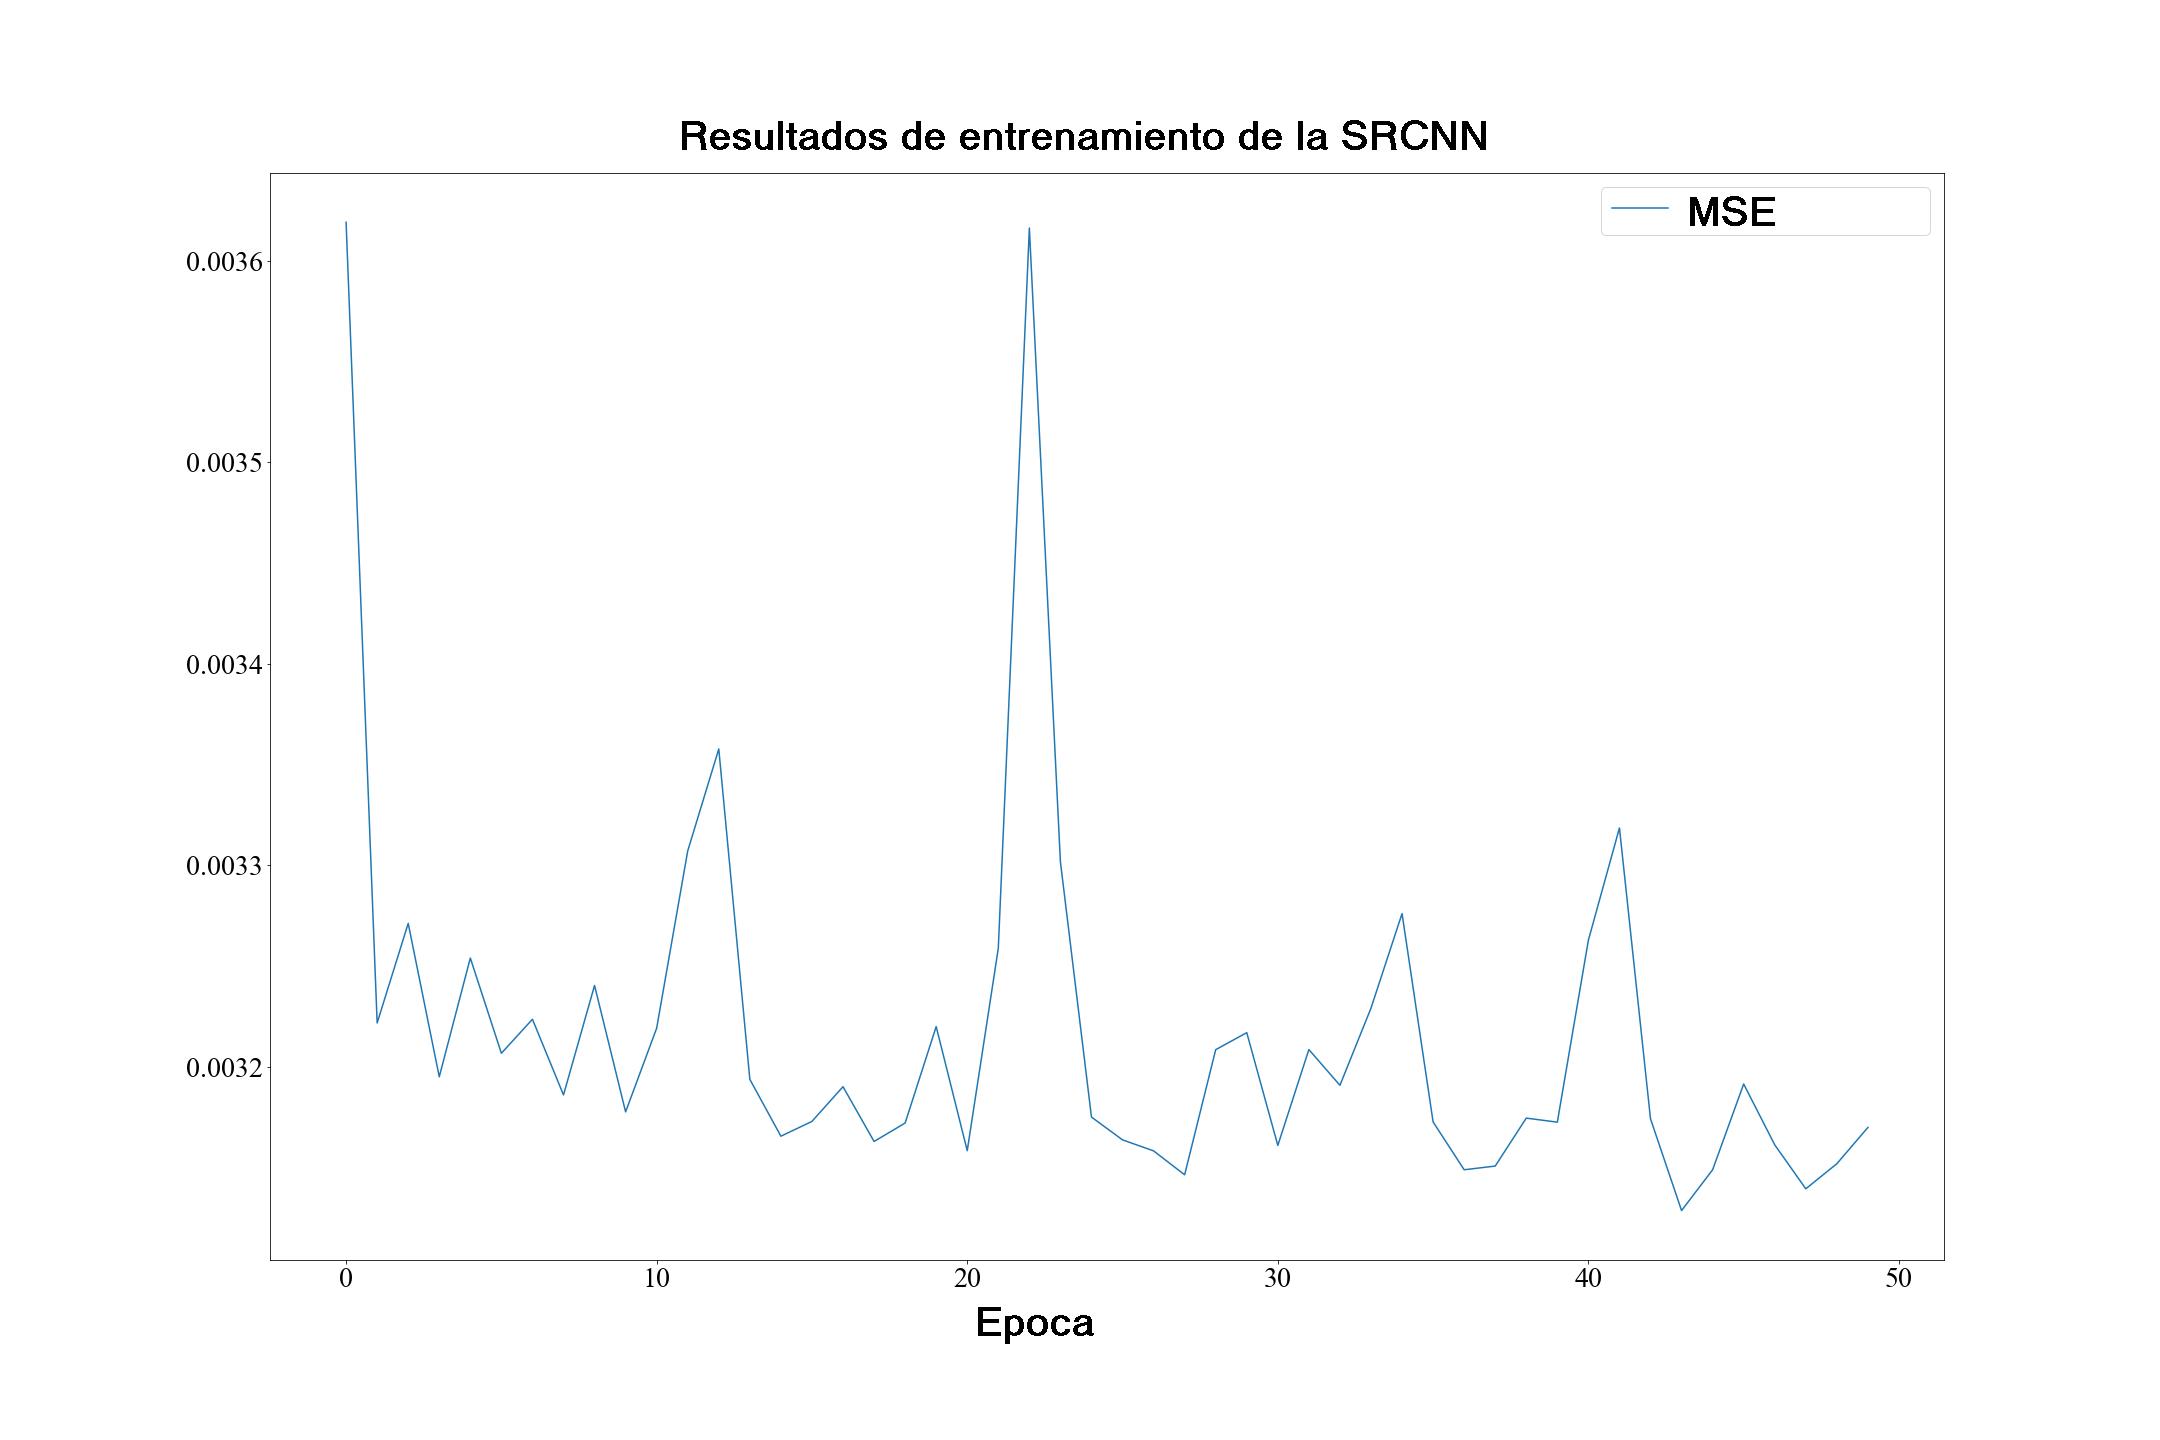
\includegraphics[width=10cm, height=6cm]{TrainingHistory_2475-2525_epochs_4RGB.png}
    \caption{Minimización de función de costo (MSE) de red convolucional}
\end{figure}

Se observa 